\section{Experimental results}
% Bigger picture
In per-pixel classification, there are many parameters involved in capturing the training images, extracting features, and training the random forest classifier. To study the contribution of these parameters, we systematically varied them and studied the accuracy of the resulting classifier. To study the accuracy, we set aside a collection of images as the test set and trained on a different set of images. We didn't use cross-validation due to the time constraints in training a random forest; it would have taken considerably longer time to test the cross validation accuracy and would  have prevented us from running as many tests as we did.
% Parameters tested
We collected images of four different gestures shown in figure~\ref{fig:gestures}. We refer to each image that we captured as a ``training sample''. Since there are over 300000 pixels in each image, we sampled only 2000 of them so that we can train on more diverse images. From each image, we sampled 1000 background points, and 1000 points from the gesture to ensure we trained evenly on the different types of classes.
\subsection{Varying Parameters} 
We varied three parameters in training the models, such the number of trees, the number of features, and the number of training samples. We set aside 50 images as the test set, on which we evaluate the trained model to obtain test accuracy. 

\textbf{Number of trees.} Figure~\ref{fig:varytrees} shows the results of varying the number of trees while fixing the remaining parameters. We observed that the number of trees makes no noticeable difference. In fact, even training the forest with one tree has the same accuracy as with multiple trees. This was also observed for different fixed values of the parameters. Adding multiple trees in the random forest is intended to protect against overfitting. However, our test and training sets were sampled from the same pool of images so we hypothesize one tree is sufficient to model all the variability in the test set. In the actual system, we used 3 trees to make the tradeoff between enough generality of the random forest and efficient performance. 

\textbf{Number of training samples.} Figure~\ref{fig:largetraining} shows the effect of varying the number of training samples. There is a clear trend of smaller test error as we increase the number of training samples. At 689 training samples, the error is only 1.32\%. Increasing the number of training samples had the biggest impact in reducing the error when compared to other factors. 

\textbf{Number of features.} Figure~\ref{fig:varyfeatures} shows the effect of varying the number features. Across most of our experiments we observed that using 2000 features outperforms 3000 features, which outperforms 1000 features. However, as seen in figure~\ref{fig:varyfeatures}, the difference in error is small. This suggests that if we sampled 1000, 2000, and 3000 features again, we may observe a different trend.

\textbf{Varying $R_{\text{max}}$}
Finally, Figure~\ref{fig:varyradii} shows the results of varying $R_{\text{max}}$ in Eq~(\ref{eqn: radius}), the radius of the offset features. For smaller training sample sizes, setting the radius to 40000 mmpx gives the least error classifier. However, as we increase the number of training samples, both 40000 mmpx and 80000 mmpx give similarly accurate classifiers. This means that when we have fewer training samples, setting the radius to 40000 mmpx will allow us to train a more accurate classifier, but when we have enough training samples, the radius is not so important. We notice that making the radius too small or too large gives poor accuracy. By qualitatively checking the offset images as shown in Figure~\ref{fig:offset}, we hypothesize that to train a more accurate classifier, the offsets should cover most of the hand, and then some of the background. If the radius is too small, then the offsets will be right next to each other and feature vectors for different gestures may be too similar.

\subsection{ Randomness }
First, due to the nature of the random forest (because of bootstrapping), the trained model is non-deterministic and may yield a different accuracy rate for the same training set of images. In order to study this randomness, we trained ten models on the same training set with 1000 features, 300 training images, and one tree. We obtained a mean error of 9.82\% with 0.94\% standard deviation. Therefore we concluded that the randomness derived from the random forest is negligible. 

\subsection{ SVM Comparison}
We compared random forest classifier with a linear SVM classifier, \cite{liblinear}. We trained an SVM classifier for 2000 features, and different number of training images. 
Figure~\ref{fig:linearsvm} compares the error rate of a linear SVM with a random forest classifier. Linear SVM only slightly outperforms a random classifier that always predicts a pixel as the background. As we increase the training sample size, linear SVM improves much more slowly than the random forest.

\subsection{Pruning}
We studied the effect of pruning on the accuracy of prediction. To study this, we pruned the forests trained with 2000 features and three trees for different number of training images. Then we calculated the test set accuracy of the pruned models. It turned out that pruning the tree showed almost no difference in accuracy compared to the full tree. We hypothesize the reason for this is that very high up in the tree the splitting nodes already confidently divide the training points into their class. However, the random forest algorithm continues to exhaust the features until the entire tree is constructed. By stopping the prediction early on in the tree, we do not suffer in accuracy, and improve the speed of prediction.


\subsection{Overfitting}
Finally, we studied how much the model overfits to the training samples by calculating the training accuracy and comparing that with the test accuracy. We fixed 2000 features and three trees and varied the number of training samples. Figure~\ref{fig:trainingacc} shows evidence of extreme overfitting. The training error is consistently very low (mean 1.06\%) and is much lower than the testing accuracy. 

\begin{figure*}
\centering
  \subfloat[Varying the number of trees. Number of feature: 2000.] {
  \label{fig:varytrees}
  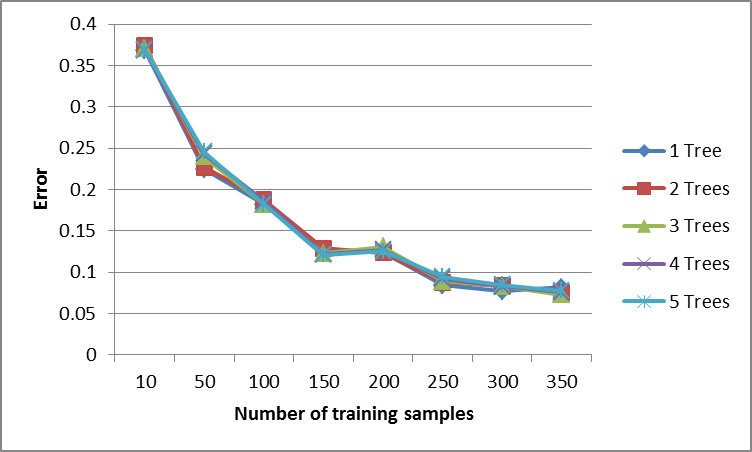
\includegraphics[width=0.3 \textwidth]{fig/varytrees.png}
  }  
  ~
  \subfloat[Varying number of training samples. 
Number of features: 2000, and number of trees: 3.]{
  \label{fig:largetraining}
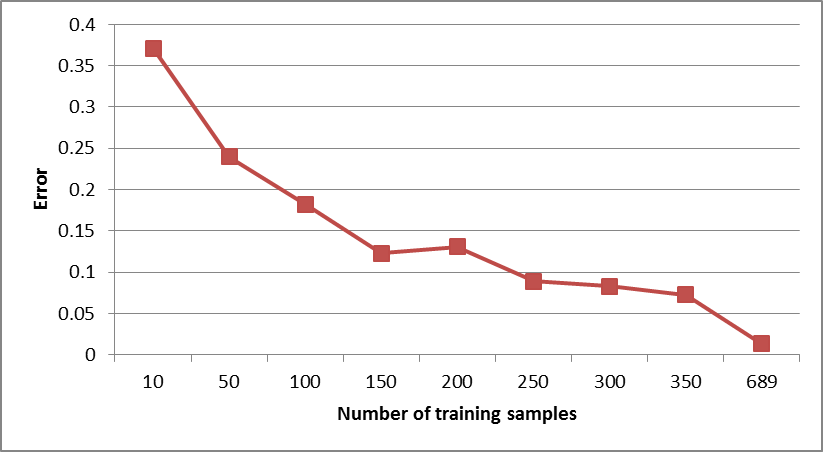
\includegraphics[width=0.3 \textwidth]{fig/largetraining.png}  
  }
  ~ 
  \subfloat[Varying the number of features. Number of trees: 3.]{
  \label{fig:varyfeatures}
  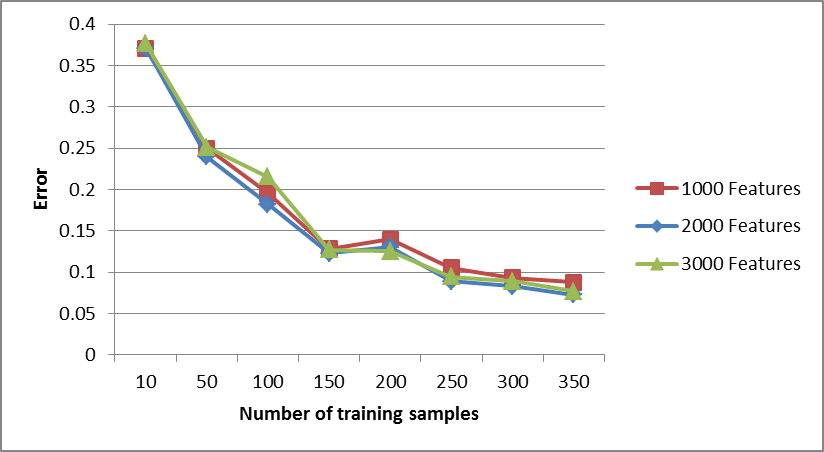
\includegraphics[width=0.3 \textwidth]{fig/varyfeatures.png}
   }
   
  \subfloat[Varying the radius of offsets. Number of features: 2000,  number of trees: 3.]{
  \label{fig:varyradii}
  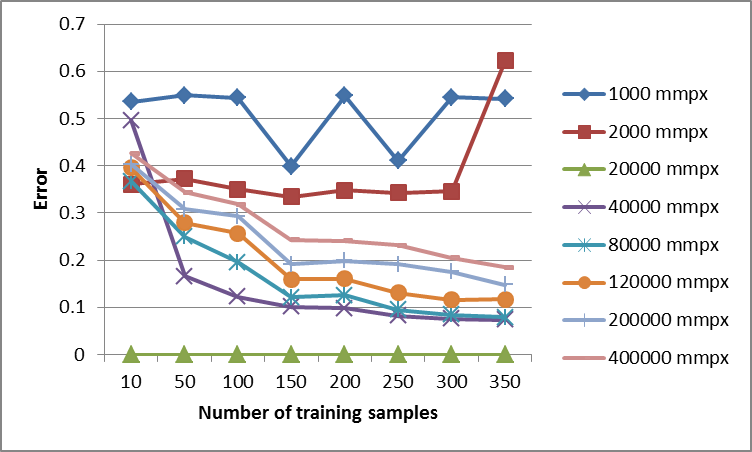
\includegraphics[width=0.3 \textwidth]{fig/varyradii.png}
  }
  ~
  \subfloat[Comparing random forest to linear SVM. Number of features: 2000,  number of trees: 3.]{
  \label{fig:linearsvm}
  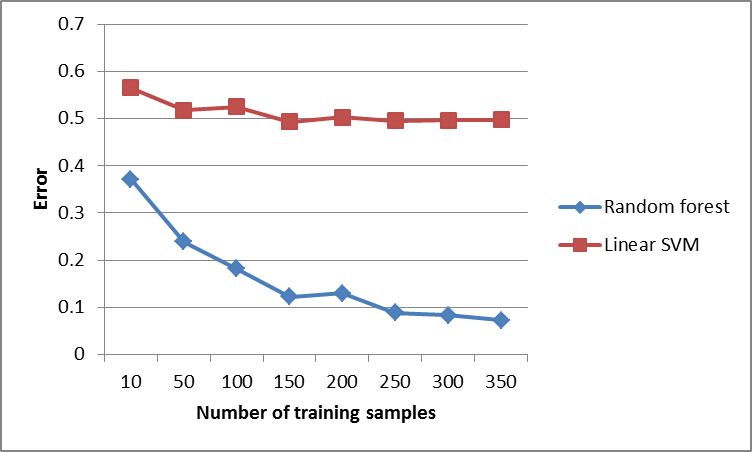
\includegraphics[width=0.3 \textwidth]{fig/linearsvm.png}
  }  
  ~	
  \subfloat[Comparing training error and testing error. Number of features: 2000,  number of trees: 3.]{
  \label{fig:trainingacc}
  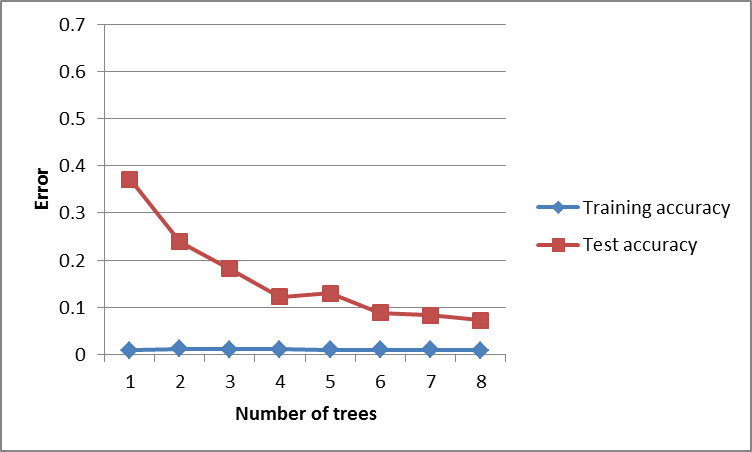
\includegraphics[width=0.3 \textwidth]{fig/trainingacc.png}
  }     
%  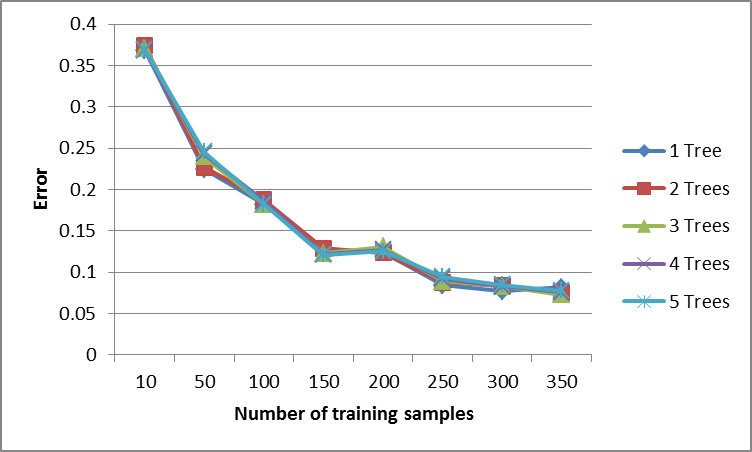
\includegraphics[width=0.45 \textwidth]{fig/varytrees.png}
%  \caption{Testing error with respect to the number of trees and the number of training samples. We fixed the number of feature to 2000.}
%  \label{fig:varytrees}
%  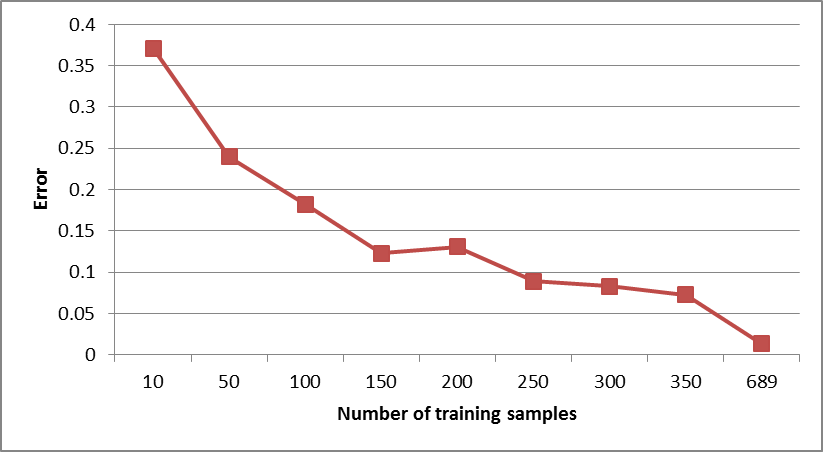
\includegraphics[width=0.45 \textwidth]{fig/largetraining.png}
%%\end{center}
%  \caption{Testing error with respect of the number of training samples. 
%%We fixed the number of features to 2000, and the number of trees to 3.}
%  \label{fig:largetraining}
  \label{fig: expfig}
\caption{Experimental results. Testing error with respect to the number of training samples.}	 
\end{figure*}


%\begin{figure}
%\begin{center}
%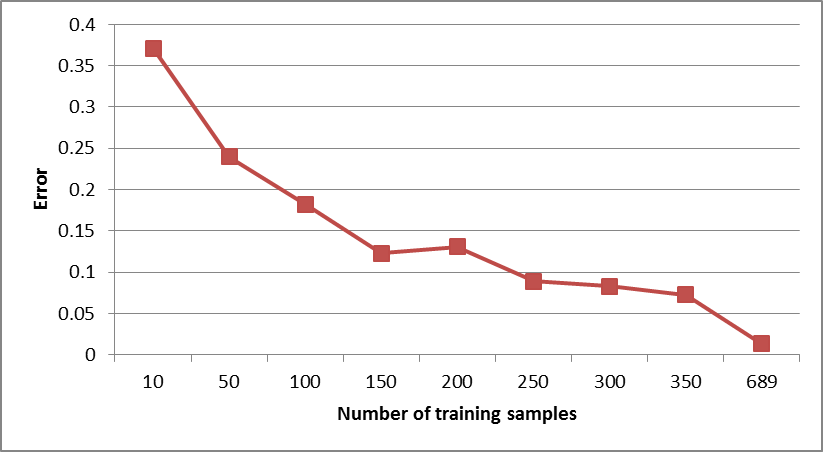
\includegraphics[width=0.45 \textwidth]{fig/largetraining.png}
%\end{center}
%\caption{Testing error with respect of the number of training samples. 
%We fixed the number of features to 2000, and the number of trees to 3.}
%\label{fig:largetraining}
%\end{figure}

%\begin{figure}
%\begin{center}
%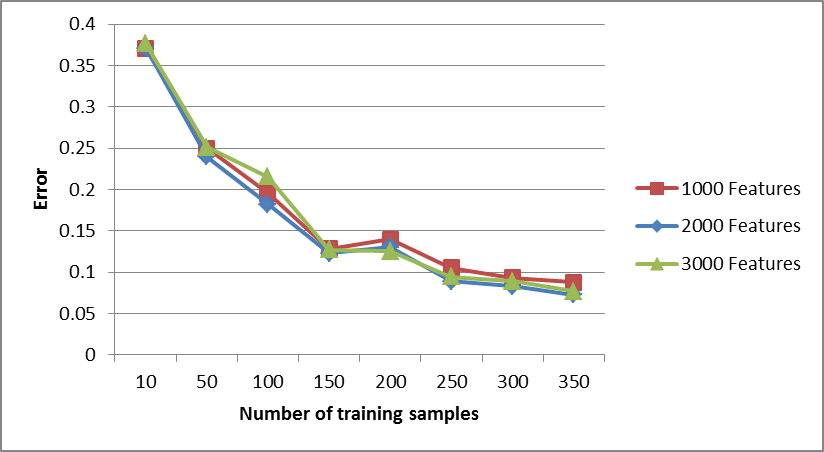
\includegraphics[width=0.45 \textwidth]{fig/varyfeatures.png}
%\end{center}
%\caption{Testing error with respect of the number of features and number of training samples. We fixed the number of trees to 3.}
%\label{fig:varyfeatures}
%\end{figure}

%\begin{figure}
%\begin{center}
%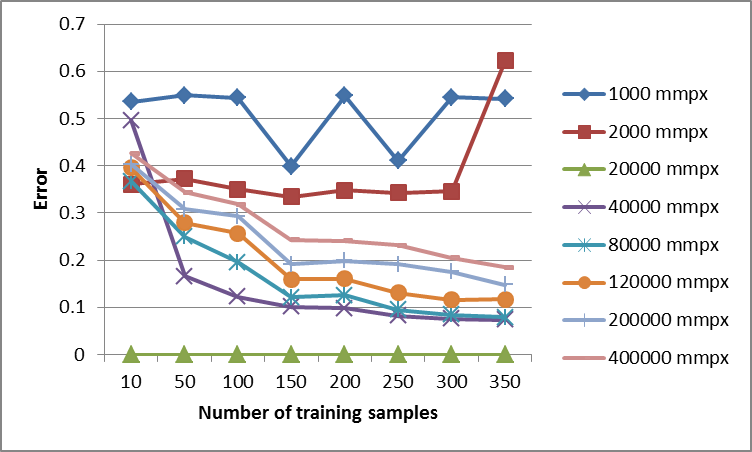
\includegraphics[width=0.45 \textwidth]{fig/varyradii.png}
%\end{center}
%\caption{Test error with respect of the radius of offsets. We fixed the number of features to 2000, and number of trees to 3.}
%\label{fig:varyradii}
%\end{figure}
%\begin{figure}
%\begin{center}
%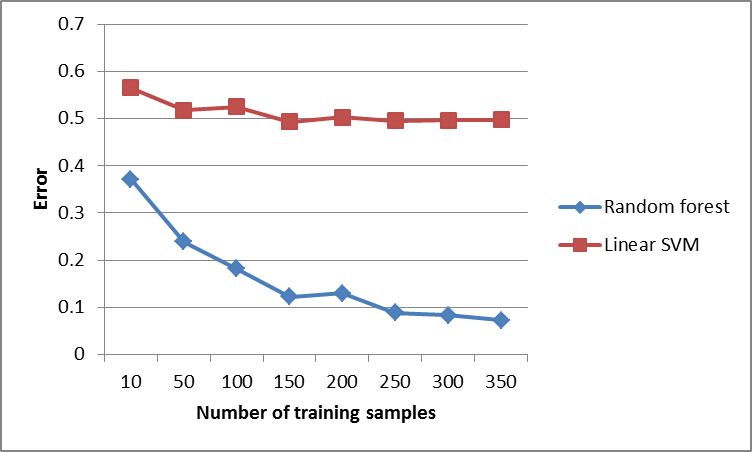
\includegraphics[width=0.45 \textwidth]{fig/linearsvm.png}
%\end{center}
%\caption{Comparing random forest to linear SVM. We fixed the number of features to 2000, and number of trees to 3. }
%\label{fig:linearsvm}
%\end{figure}
%
%\begin{figure}
%\begin{center}
%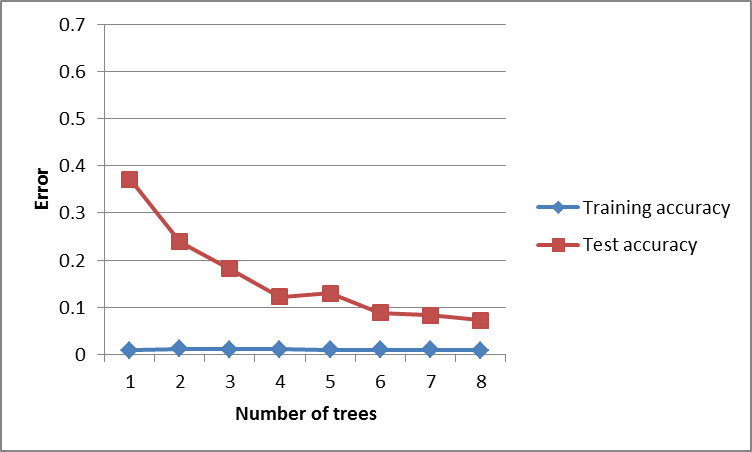
\includegraphics[width=0.45 \textwidth]{fig/trainingacc.png}
%\end{center}
%\caption{Comparing training error and testing error. We fixed the number of features to 2000 and the number of trees to 3..}
%\label{fig:trainingacc}
%\end{figure}
